\subsection{Bestimmung der Flächenträgheitsmomente}
Das Flächenträgheitsmoment ist eine Größe, die im weiteren Verlauf wichtig ist, um den Elastizitätsmodul der Stäbe zu ermitteln.
Er hängt vom Querschnitt des Stabes, genauer vom Abstand $y$ der Flächenelemente d$q$ zur neutralen Faser, ab
\begin{equation}
I = \int_{Q} y ^2 \, \text{d}q \quad .
\end{equation}
Für den eckigen Stab benötigt man eine Formel für quadratische Querschnitte. Die Kantenlänge sei $h$. Für $I_\text{E}$ gilt:
\begin{equation}
I_\text{E} = \int_{-\frac{h}{2}}^{\frac{h}{2}} \int_{-\frac{h}{2}}^{\frac{h}{2}} y^2\,  \text{d}x \text{d}y = \frac{1}{12} \cdot h^4 \quad .
\end{equation}
Um das Flächenträgheitsmoment für runde Querschnitte mit Radius $r$ zu berechnen, bietet sich die Verwendung von Polarkoordinaten an. Der Abstand zur $y$-Achse ist dann $r^2 \cdot \sin^2(x)$.  Mit der Jakobideterminante $r$ ist $I_R$
\begin{equation}
I_\text{R} = \int_{0}^{r}  \int_{0}^{2\pi} r^2 \cdot \sin^2(x) \cdot r  \, \text{d}\phi \text{d}r = \frac{1}{12}\cdot \pi \cdot r^4 \quad .
\end{equation}
Sowohl $h$ als auch der Durchmesser $2 \cdot r$ wurden sehr genau mit einer Schieblehre gemessen. Zum Fehler des Mittelwertes kommt ein Ablesefehler von \SI{0.05}{\milli\metre} dazu.

\begin{center}
	\captionof{table}{Breite $h$ des eckigen Stabes und Durchmesser $2 \cdot r$ des Runden}
\begin{tabular}{c|c}
	Breite $h$ in \SI{}{\milli\metre}& Durchmesser $2 \cdot r$ in \SI{}{\milli\metre}	\\
	\hline
	10.00 & 10.00 \\
	10.00  & 10.00 \\
	10.00  & 10.00 \\
	10.00  & 9.90 \\
	10.00  & 9.90 \\
	10.00  & 9.95 \\
	10.00  & 10.00 \\
	10.00  & 9.90 \\
	10.00  & 9.90 \\
	10.00 & 9.95 \\
\end{tabular}	
\end{center}

Für den eckigen Stab folgt mit dem Mittelwert der Breite
\begin{align}
  h = \SI{0.01000 \pm 0.00005}{\metre}
\end{align}
ein Flächenträgheitsmoment von
\begin{align}
I_\text{E}=\SI{3.88(17)e-10}{\metre\raiseto{4}} \quad .
\label{I_E}
\end{align}

Für den runden Stab folgt mit einem Radius von
\begin{equation}
  r = \SI{0.004975 \pm 0.000032}{\metre}
\end{equation}
das Flächenträgheitsmoment
\begin{equation}
  I_\text{R} = \SI{4.81(12)e-10}{\metre\raiseto{4}} \quad .
  \label{I_R}
\end{equation}


\subsection{Bestimmung des Elastizitätsmodul durch lineare Regression}
\subsubsection{Runder Stab -- einseitige Einspannung}
Die gemessene Durchbiegung $D(x)$ des Stabes wird durch die Gleichung \eqref{einseitige Einspannung} beschrieben.
Alle in ihr vorkommende Größen, bis auf das Elaatizitästmodul sind bekannt. Das Flächenträgheitsmoment wurde im vorherigen Abschnitt als \eqref{I_R} bestimmt und die herabziehende Kraft $F$ ist aus der Masse des Probekörpers zu berechnen
\begin{equation}
  F = m \cdot g = \SI{0.7476}{\kilo\gram} \cdot \SI{9.81}{\metre\per\second\squared} = \SI{7.3339}{\newton} \quad .
\end{equation}
Nun lässt sich das Elastizitäsmodul $E$ druch eine lineare Regression der Form
\begin{equation}
  D(x) = \frac{F}{2\cdot E I}\left(Lx^2-\frac{x^3}{3}\right) = \frac{1}{E} \cdot A +b
\end{equation}
bestimmen, indem $D(x)$ über $A$ ausgetragen wird (siehe Abbildung \ref{fig:Regression_runder_Stab}). $E$ entspricht dem Kehrwert der Steigung der Regressionsgeraden. Unter Verwendung der Formeln aus Kapitel~\ref{sec:regression} ergibt die Steigung mit Abweichung
\begin{equation}
  \frac{1}{E}= \SI{188.9(15)e-13}{\metre\squared\per\newton}
\end{equation}
und der $y$-Achsenabschnitt mit Abweichung
\begin{equation}
  b = \SI{14.33(36)e-05}{\metre} \quad.
\end{equation}
Das hier bestimmte Elastizitästmodul für den runden Stab ist folglich
\begin{equation}
  E = \SI{5.29(4)e+10}{\newton\per\metre\squared} \quad.
\end{equation}

\begin{figure}
\centering
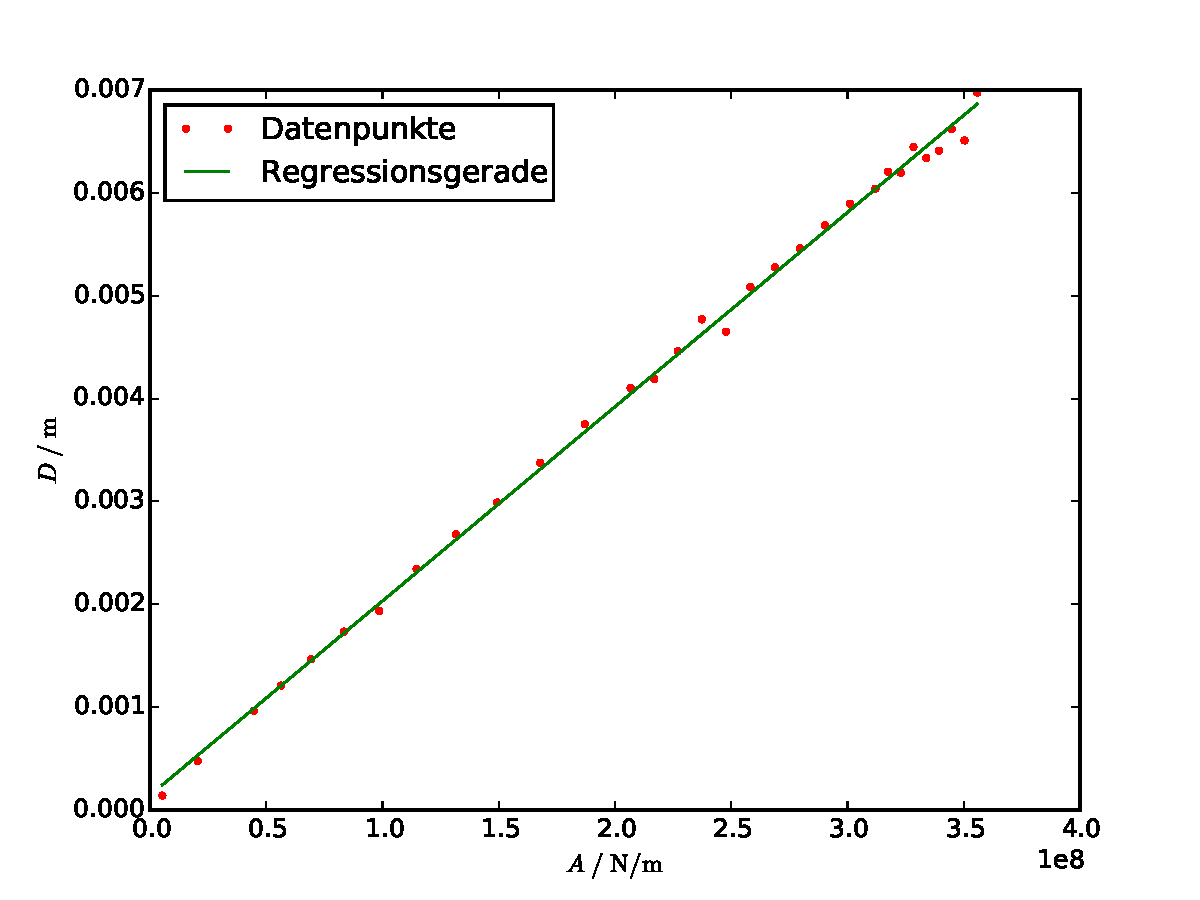
\includegraphics[width=\textwidth]{Regression_runder_Stab.pdf}
\caption{Regressionsgerade des runden Stabes bei einseitiger Einspannung}
\label{fig:Regression_runder_Stab}
\end{figure}



\subsubsection{Eckiger Stab -- einseitige Einspannung}
Hier ist der Vorgehensweise genau so, wie bei dem runden Stab. Es muss lediglich ein anderes Flächenträgheitsmoment \ref{I_E} und eine andere Kraft
\begin{equation}
  F = m \cdot g = \SI{0.7676}{\kilo\gram} \cdot \SI{9.81}{\metre\per\second\squared} = \SI{7.5302}{\newton}
\end{equation}
eingesetzt werden.
Dies führt auf eine Steigung mit Abweichung von
\begin{equation}
  \frac{1}{E}= \SI{135.6(9)e-13}{\metre\squared\per\newton}
\end{equation}
und den $y$-Achsenabschnitt mit Abweichung
\begin{equation}
  b = \SI{6.28(217)e-05}{\metre} \quad.
\end{equation}
Das hier bestimmte Elastizitästmodul für den eckigen Stab ist folglich
\begin{equation}
  E = \SI{7.37(5)e+10}{\newton\per\metre\squared} \quad.
\end{equation}
Die Werte wurden in Abbildung~\ref{fig:Regression_eckiger_Stab} aufgetragen.

\begin{figure}[h!]
\centering
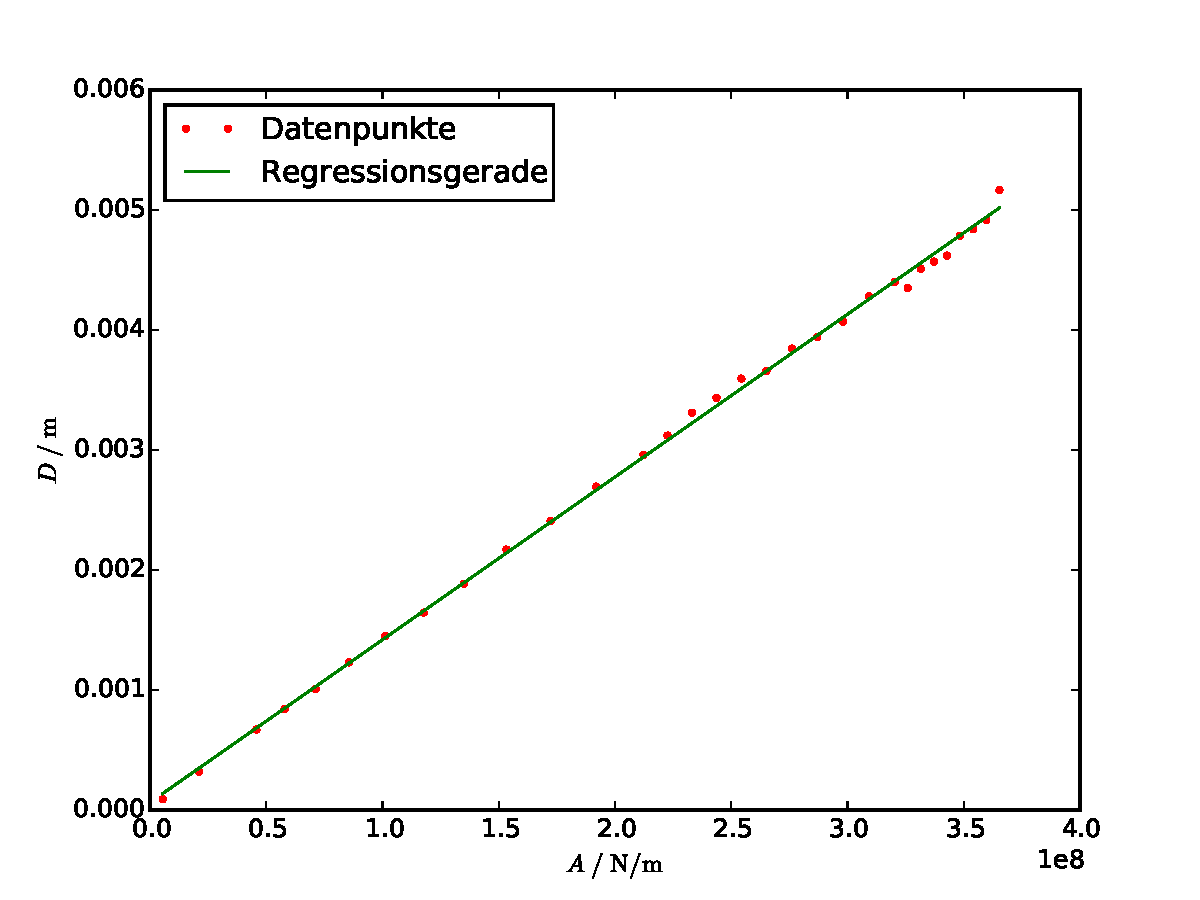
\includegraphics[width=\textwidth]{Regression_eckiger_Stab.pdf}
\caption{Regressionsgerade des eckigen Stabes bei einseitiger Einspannung}
\label{fig:Regression_eckiger_Stab}
\end{figure}







\subsubsection{Eckiger Stab -- beidseitige Einspannung}
Die Bestimmung des Elastizitätsmoduls bei beidseitiger Einspannung ist ähnlich zu der bei einseitiger. Sie unterscheidet sich in der Ausführung im Wesentlichen durch die minimal andere Formel \ref{beidseitige Einspannung}, eine andere Kraft, da ein schwereres Gewicht verwendet wurde
\begin{equation}
  F = m \cdot g = \SI{4.7004}{\kilo\gram} \cdot \SI{9.81}{\metre\per\second\squared} = \SI{46.1109}{\newton}
\end{equation}
und die Tatsache, dass links und rechts von dem in der Mitte eingehängten Gewicht die Verbiegung des Stabes gemessen wurde. Es gibt zwei Regressiongeraden: Eine für die Werte links vom Stab und die andere für die rechte Seite. \\
Zunächst soll die Regressionsgerade der linken Seite betrachtet werden. Sie hat eine Steigung mit Abweichung von
\begin{equation}
  \frac{1}{E}= \SI{55.45(188)e-13}{\metre\squared\per\newton}
\end{equation}
und den $y$-Achsenabschnitt mit Abweichung von
\begin{equation}
  b = \SI{44.5(23)e-05}{\metre} \quad.
\end{equation}
Daraus folg das Elastizitätsmodul
\begin{equation}
  E = \SI{18.0(6)e+10}{\newton\per\metre\squared} \quad.
\end{equation}
\\
Für die rechte Seite ergeben sich Werte von
\begin{align}
  \frac{1}{E} &= \SI{72.25(303)e-13}{\metre\squared\per\newton} \quad,\\
  b &= \SI{30.6(47)e-05}{\metre} \\
  \intertext{und}
  E &= \SI{13.8(6)e+10}{\newton\per\metre\squared} \quad.
\end{align}

\begin{figure}
\centering
\begin{subfigure}{0.49\textwidth}
\centering
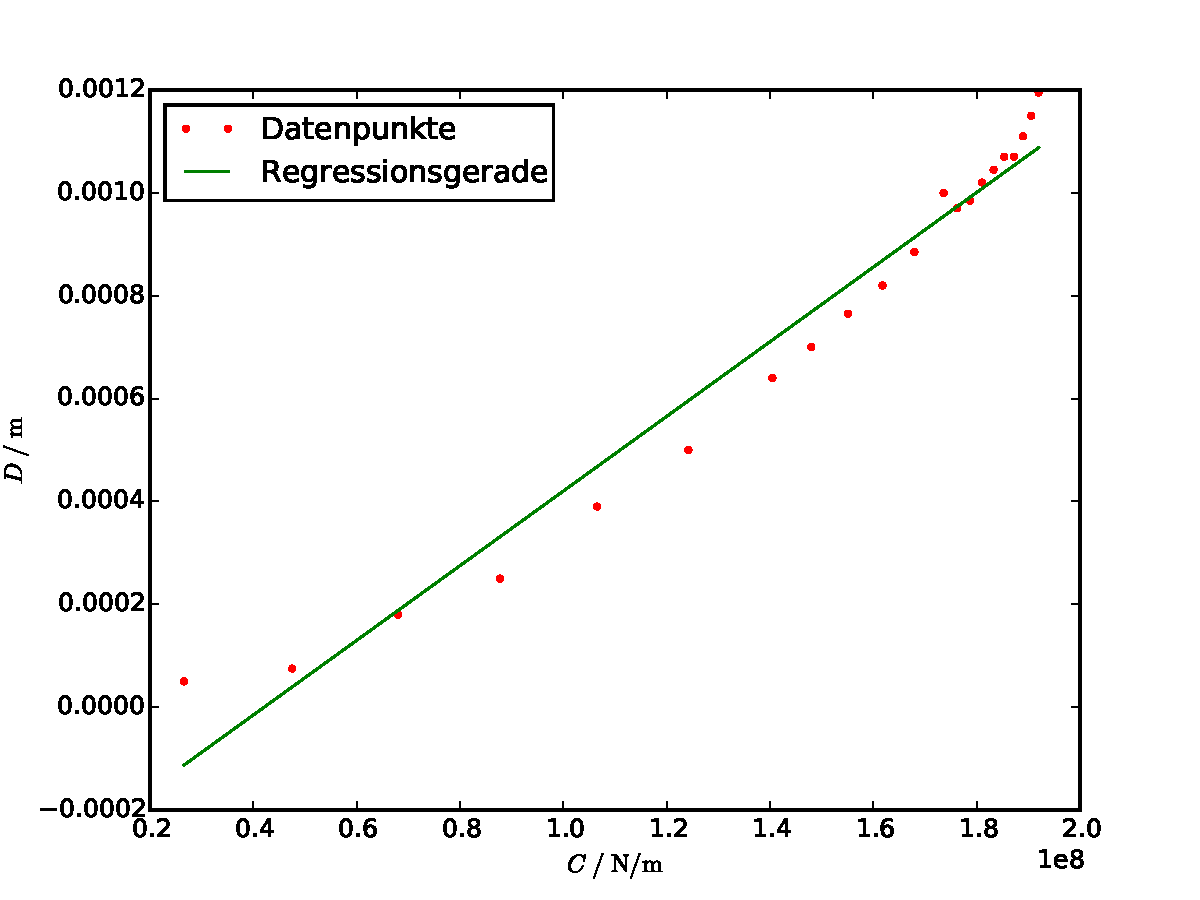
\includegraphics[width=\textwidth]{Regression_zweiseitig_eingespannt_1.pdf}
\caption{Linke Seite}
%\label
\end{subfigure}
\begin{subfigure}{0.49\textwidth}
\centering
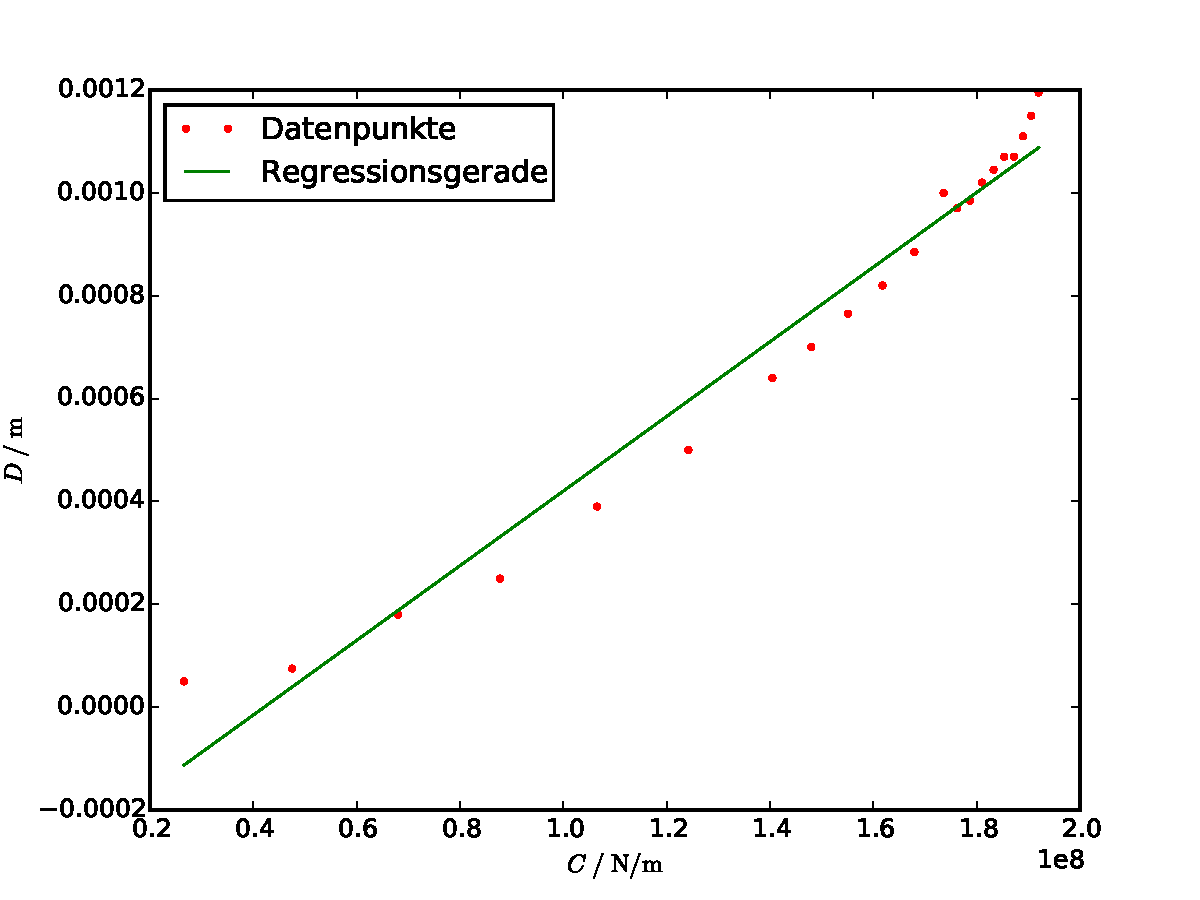
\includegraphics[width=\textwidth]{Regression_zweiseitig_eingespannt_2.pdf}
\caption{Rechte Seite}
%\label
\end{subfigure}
\caption{Regressionsgerade des eckigen Stabes bei beidseitiger Einspannung}
%\label{fig:logos}
\end{figure}


\subsection{Bestimmung der Dichte}
<<<<<<< HEAD
Zur Bestimmung der Dichte wurden beide Stäbe , der runde und der eckige, vermessen und gewogen. Das Gewicht und die Länge sind keine fehlerbehafteten Größen. Der Durchmesser hingegen wurde mit einer Schieblehre mehrfach gemessen. Ein Ablesefehler von \SI{0.05}{\milli\metre}  kommt zu dem Fehler des Mittelwertes hinzu.
Zur genaueren Festlegung, aus welchen Metallen die Stäbe bestehen können, ist die Dichte wichtig. Zur Berechnung der Dichte sind die Ausmaße der Stäbe und ihr Gewicht wichtig.
Der Querschnitt bzw. Radius der Stäbe wurde (Werte in Tabelle \ref{tab:querschnitte}) bereits als fehlerbehaftete Größe bestimmt. In Länge und das Gewicht haben keine angegebenen Ungenauigkeiten. \\
Die Dichte ist jeweils
\begin{equation}
  \rho = \frac{\text{Gewicht}}{\text{Querschnittsfläche} \cdot \text{Länge}} \quad.
\end{equation}
Der runde Stab der Länge \SI{0.6}{\metre} ist \SI{0.3945}{\kilo\gram} schwer und hat die Dichte
\begin{equation}
  \rho_\text{Rund} = \SI{8455.90(10902)}{\kilo\gram\per\cubic\metre} \quad.
\end{equation}  \\
Und der eckige Stab der Länge \SI{0.6}{\metre} ist \SI{0.1671}{\kilo\gram} schwer und hat die Dichte
\begin{equation}
  \rho_\text{Eckig} = \SI{2785.00(2785)}{\kilo\gram\per\cubic\metre} \quad.
\end{equation}
